%*****************************************
\chapter{Related Implementations}
\label{chapter:related_implementations}
%*****************************************

\section{HACKER}

A good precedent for reflective debugging responses to catalogs of
failures is \emph{HACKER}, one of the first reflective planning and
debugging models, written by \cite{sussman:1973}.  [complete]

\section{EM-ONE}

\cite{singh:2005b} provided \emph{EM-ONE}, a most recent example of an
extension of HACKER that reasons about a more complicated
three-dimensional physical and social block building domain.
[complete]

\section{Propagators}

\cite{radul_and_sussman:2009} describe an object called a \emph{cell}
that is closely related to the knowledge dependencies depicted in
{\mbox{\autoref{figure:dependency_traces}}}.  These cells can be
connected by dependency sets that specify functions that derive new
knowledge from the dependencies, as well as, functions for merging the
collected knowledge in cells.  Collections of Radul and Sussman's
cells are called a \emph{propagator}.  The knowledge dependencies in
this model can be thought of as a type of propagator.  The combination
of a propagator model of knowledge maintenance with a reflective
organization is described as future research in
\autoref{chapter:future}.
%\begin{figure}
%\center
%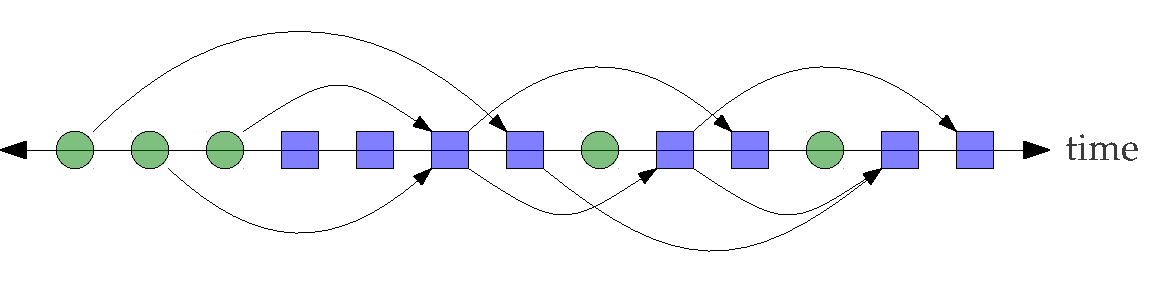
\includegraphics[width=10cm]{gfx/dependency_traces}
%\caption{Dependency traces as propagator cells.}
%\label{figure:propogators_dependency_traces}
%\end{figure}
